\documentclass[11pt]{article}
\usepackage{fullpage}
\usepackage{amsmath}
\usepackage{amssymb}
\usepackage{graphicx}
\usepackage{color}
\usepackage{float}
\usepackage{caption}
\usepackage{placeins}

\renewcommand\baselinestretch{1.5}
\newcommand{\reals}{\mathbb{R}}
\newcommand{\Pose}{{\cal P}}
\newcommand{\Active}{{\cal A}} 
\newcommand{\X}{\mathbf{X}} 
\newcommand{\symb}{\Sigma}

\begin{document}

\title{Jeroen's model}
\maketitle

\section{Notation}

\begin{itemize}

\item $\symb$: partially-ordered list of symbols (types).

\item $\symb_i$: ith symbol in partial ordering.

\item $T$: number of symbols in grammar.

\item $\Pose$: pose space.

\item $\Pose(b)$: pose cell of brick $b$- a set of poses. $\Pose(b) \in \Pose$ 

\item $\Active = (a_1,\ldots,a_M)$: set of active bricks.

\item $\Active \subseteq {\cal B}$.

\item ${\cal B} = (b_1,\ldots,b_N)$: set of bricks.

\item $t(b)$: type of brick $b$.

\item ${\cal R}$: set of production rules of the form
$A \rightarrow B_1,\ldots,B_k$ with $r = A,B_1,\ldots,B_k \in \Sigma$. ${\cal R}$ is acyclic.

\item $n(r)$: number of slots/children associated with rule $r \in {\cal R}$

%%%\item $c(b) = {\displaystyle \max_{r \in {\cal R}, LHS(r) = t(b)}} n(r): $ maximum number of slots/children associated with a brick $b$

\item $p_{r,n}(x_i|x)$, $r \in {\cal R}$, $x,x_i \in {\cal P}$, $n \in [1...n(r)]$: 
conditional probability density over pose for $B_i$ given pose for $A$ for this rule and slot.

\item ${\cal R}(A)$: rules with $A$ in the left-hand-side (LHS).

\item $p_A$: distribution over ${\cal R}(A)$.

\item $s_b \in \{0,1\}$: on/off state of brick $b$.

\item $r_b \in {\cal R}(t(b))$: rule used by brick $b$.

\item $\mathbf{g_b} \in ( {\cal B} \cup \perp )^{c(b)}$: array of pointers, where each element can either point to a brick, or null (no child).

\item $V(b)$: ``before'' set of bricks, which we define as $V(b) = \{b' : t(b') < t(b) \}$ where $<$ means ``comes before in the partial ordering defined by $\symb$''.

\item $W(b)$: ``after'' set of bricks, which we define as $V(b) = \{b' : t(b') > t(b) \}$ where $>$ means ``comes after in the partial ordering defined by $\symb$''.

\item $q_b \in \Pose(b)$: pose for brick $b$. $q_b = \perp$ is a special ``nothing'' pose that does not contribute to image evidence.

\item $\X = \{ \mathbf{s}, \mathbf{r}, \mathbf{g}, \mathbf{q}\}$: collection of hidden variables of model.

\item $I$: the image.

\end{itemize}

\section{Model}

\begin{figure}[htbp]
\begin{center}
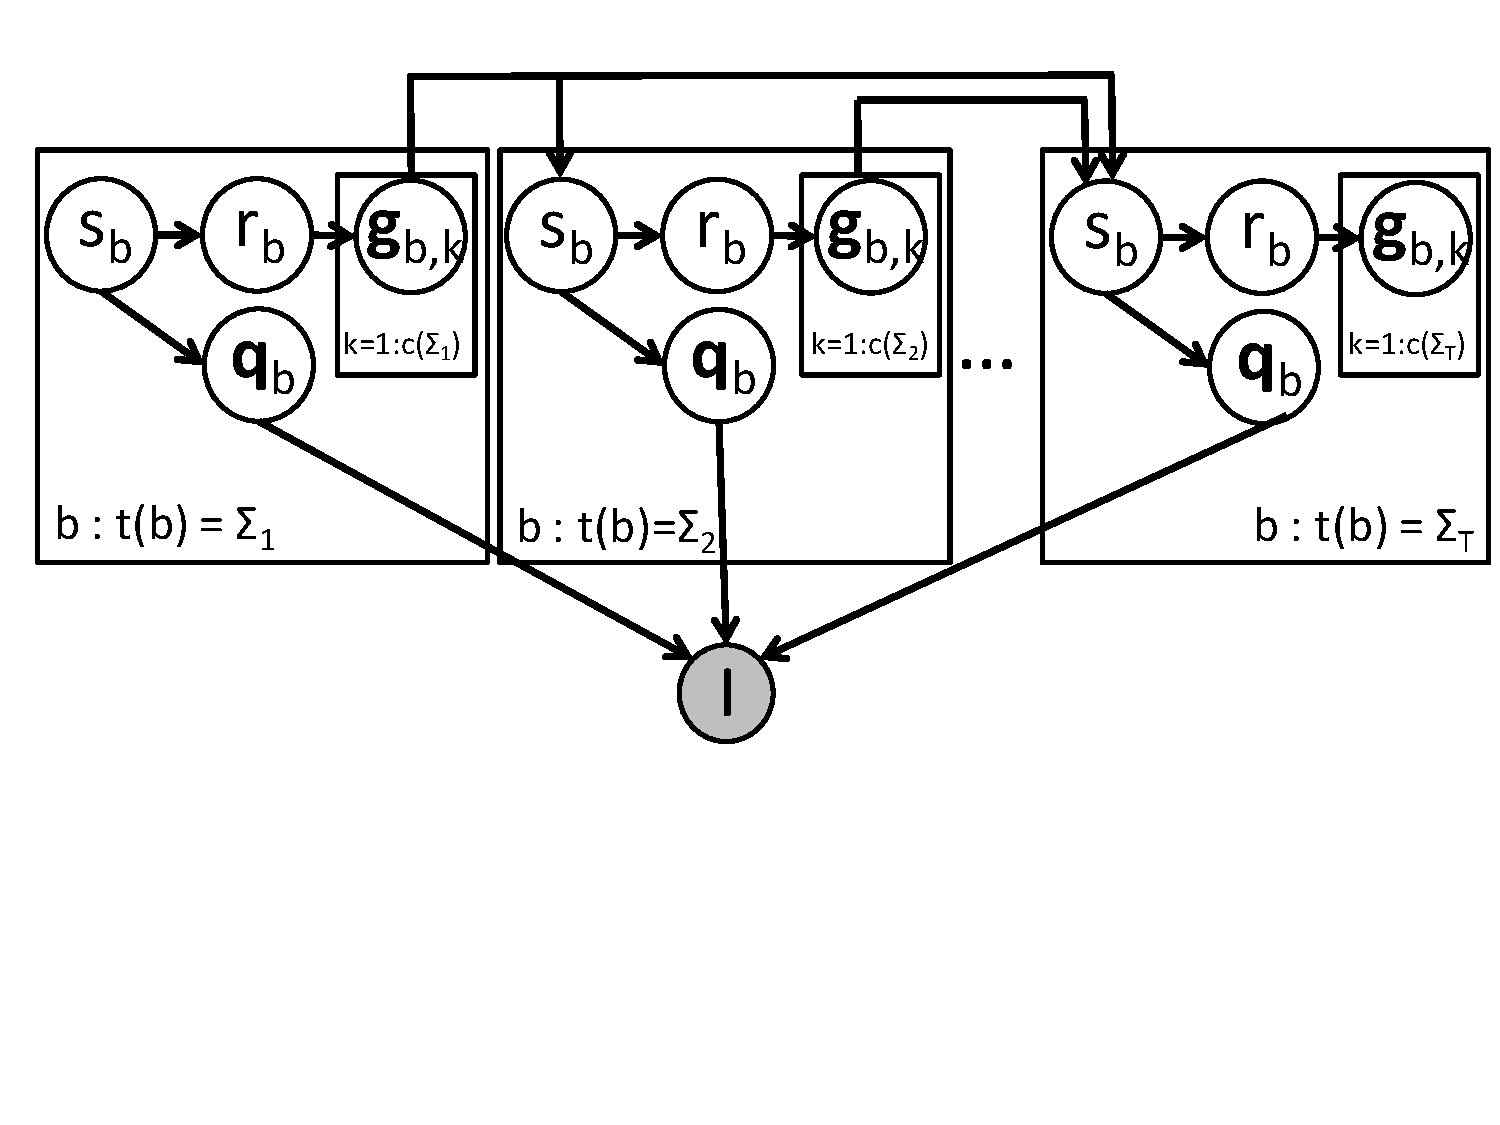
\includegraphics[width=\textwidth, trim=0cm 6cm 0cm 0cm]{gm.pdf}
\caption{Graphical model}
\end{center}
\end{figure}

\FloatBarrier

Joint probability is given by: \\

\begin{eqnarray}
P(\X, I) &=& \big({\displaystyle \prod_{b \in {\cal B}}} P(s_b \mid \mathbf{g}_{V(b)}) \big ) \\
& &\big( {\displaystyle \prod_{b \in {\cal B}}} P(r_b \mid s_b) {\displaystyle \prod_{k=1}^{c(b)}} P(g_{b,k} \mid r_b) \big) \\
& &\big( {\displaystyle \prod_{b \in {\cal B}}} P(\mathbf{q_b} \mid s_b)\big) \\
& & P(I \mid \mathbf{q})
\end{eqnarray}

Before we define localizations, we first define additional notation to ease the presentation.

\begin{itemize}
\item $\mathbf{g}_b^{\Active} \in ( {\cal A} \cup \emptyset )^{c(b)}$: array of pointers, where each element can either point to a brick, or blank (child not yet specified). Note that blank is \textbf{different} than null (no child) in that blank means ``there could be a child in this slow, but we don't know if there is or which one yet'' while null (no child) means ``there definitely isn't a child in this slot''.
\end{itemize}

For localization, we do not explicitly represent $\mathbf{r}$; instead we express the state configuration in terms of $\mathbf{g}_b^{\Active}$ only, which implicitly specifies a set of compatible rules. Rather than selecting specific values for $\mathbf{r}$, we instead marginalize over the set of compatible rules defined by $\mathbf{g^{\Active}}$ wherever  $\mathbf{r}$ is referred to.

We define localizations in terms of the components $\big({\displaystyle \prod_{b \in {\cal B}}} P(s_b \mid \mathbf{g}_{V(b)}) \big )$, $\big( {\displaystyle \prod_{b \in {\cal B}}} P(r_b \mid s_b) {\displaystyle \prod_{k=1}^{c(b)}} P(g_{b,k} \mid r_b) \big)$, $\big( {\displaystyle \prod_{b \in {\cal B}}} P(\mathbf{q_b} \mid s_b)\big)$, and $P(I \mid \mathbf{q})$ separately.

\begin{eqnarray}
\big({\displaystyle \prod_{b \in {\cal B}}} P(s_b \mid \mathbf{g}_{V(b)}) \big ) &\Rightarrow& \big({\displaystyle \prod_{a \in {\cal A}}} P^{\Active}(s_a \mid \mathbf{g}^{\Active}_{V({b})}) \big )
\end{eqnarray}

where $\Rightarrow$ is used to mean ``localiizes to''. Similarily, 

\begin{eqnarray}
\big( {\displaystyle \prod_{b \in {\cal B}}} P(r_b \mid s_b) {\displaystyle \prod_{k=1}^{c(b)}} P(g_{b,k} \mid r_b) \big) &\Rightarrow& \big( {\displaystyle \prod_{a \in {\cal A}}} \sum_{r_a} P^{\Active}(r_a \mid s_a) P^{\Active}{\displaystyle \prod_{k=1}^{c(b)}} P^{\Active}(g_{a,k} \mid r_a) \big) \\
P^{\Active}(g_{a,k} \mid r_a) &=& \textnormal{defn here. split empty, not-empty cases}
\end{eqnarray}


\begin{eqnarray}
\big( {\displaystyle \prod_{b \in {\cal B}}} P(\mathbf{q_b} \mid s_b)\big) \Rightarrow \big( {\displaystyle \prod_{a \in {\cal A}}} P^{\Active}(\mathbf{q_a} \mid s_a)\big)
\end{eqnarray}
\begin{eqnarray}
P(I \mid \mathbf{q}) \Rightarrow P^{\Active}(I \mid \mathbf{q^{\Active}})
\end{eqnarray}

%\begin{figure}[htbp]
%\begin{center}
%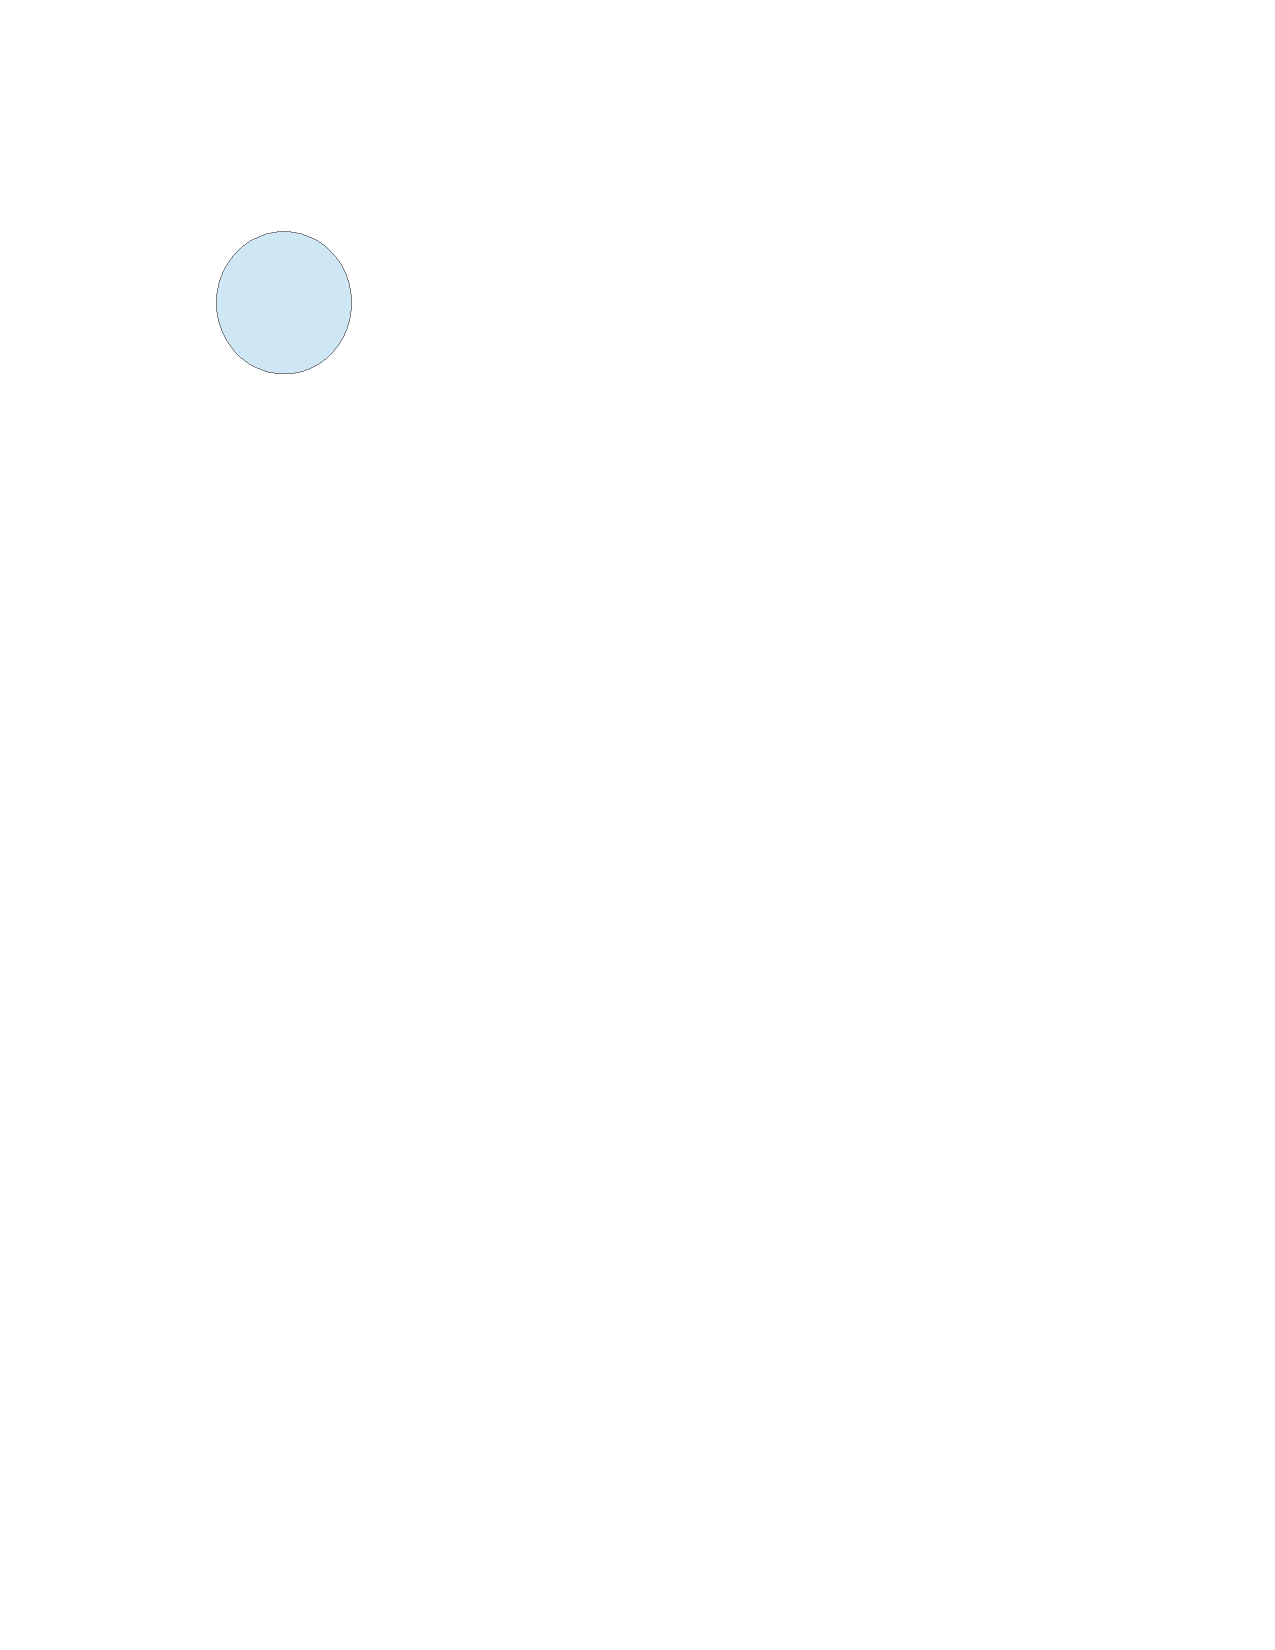
\includegraphics[width=\textwidth]{test.pdf}
%\caption{Graphical model}
%\end{center}
%\end{figure}


\end{document}
